% Copyright (c) 2017 Alexander Bluhm <bluhm@openbsd.org>
%
% Permission to use, copy, modify, and distribute this software for any
% purpose with or without fee is hereby granted, provided that the above
% copyright notice and this permission notice appear in all copies.
%
% THE SOFTWARE IS PROVIDED "AS IS" AND THE AUTHOR DISCLAIMS ALL WARRANTIES
% WITH REGARD TO THIS SOFTWARE INCLUDING ALL IMPLIED WARRANTIES OF
% MERCHANTABILITY AND FITNESS. IN NO EVENT SHALL THE AUTHOR BE LIABLE FOR
% ANY SPECIAL, DIRECT, INDIRECT, OR CONSEQUENTIAL DAMAGES OR ANY DAMAGES
% WHATSOEVER RESULTING FROM LOSS OF USE, DATA OR PROFITS, WHETHER IN AN
% ACTION OF CONTRACT, NEGLIGENCE OR OTHER TORTIOUS ACTION, ARISING OUT OF
% OR IN CONNECTION WITH THE USE OR PERFORMANCE OF THIS SOFTWARE.

\documentclass[14pt,aspectratio=169]{beamer}
%\usepackage[nomixage,puffy]{genuaslides}
\usetheme{Frankfurt}
\usepackage{tikz}
\usepackage{graphicx}

\author{Alexander Bluhm}
\title{Measuring Performance on OpenBSD}
\institute{bluhm@openbsd.org}
\date{BSDCan, May 2019}

\begin{document}

\begin{frame}
\titlepage
\end{frame}

\begin{frame}{Agenda}
\setcounter{tocdepth}{1}
\tableofcontents
\end{frame}

\section{What did exist?}

\subsection{HPF Goals}
\begin{frame}{HPF Goals}
genua Firewall Testbed

Numbers for
\begin{itemize}
    \item Customers
    \item Marketing
    \item Developers
    \item Whatever
    \item \dots
\end{itemize}
\end{frame}

\subsection{HPF Result}
\begin{frame}{HPF Result}
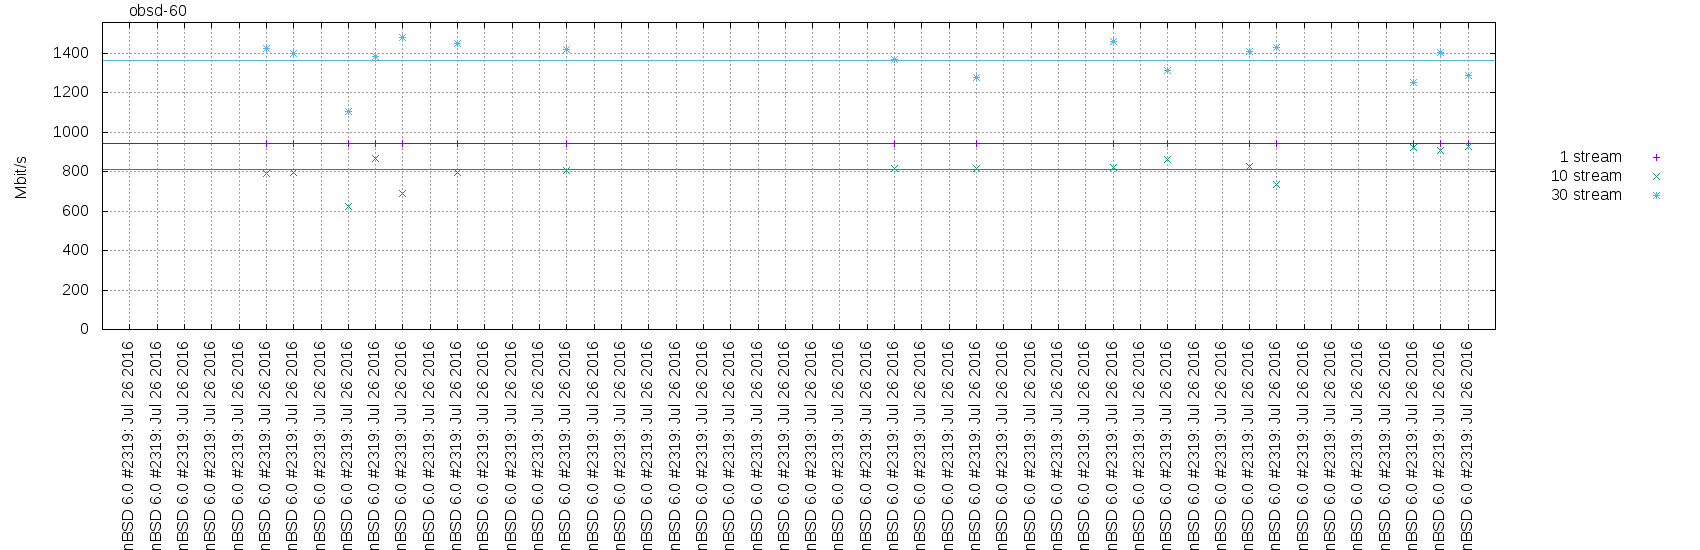
\includegraphics[width=\textwidth]{images/gs700r7_obsd_proxy_tcp.png}
\end{frame}

\subsection{Multi User Hardware}
\begin{frame}{Multi User Hardware}
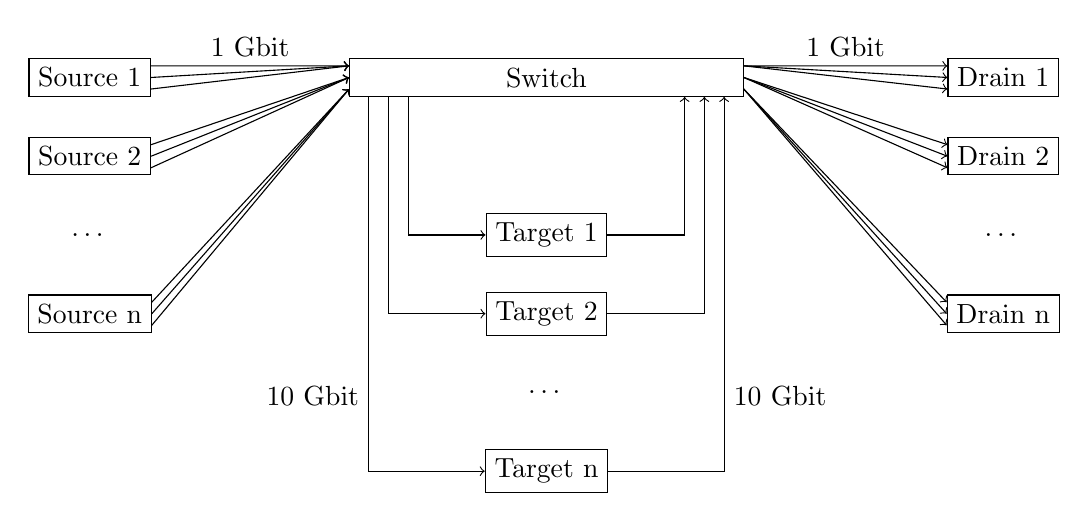
\begin{tikzpicture}
    \path (-5.8, 0) node [draw] (s1) {Source 1};
    \path (-5.8,-1) node [draw] (s2) {Source 2};
    \path (-5.8,-2) node             {\dots};
    \path (-5.8,-3) node [draw] (s3) {Source n};
    \path (s1.north east) -- (s1.south east)
     node (s11) [pos=0.2] {} node (s12) [pos=0.5] {} node (s13) [pos=0.8] {};
    \path (s2.north east) -- (s2.south east)
     node (s21) [pos=0.2] {} node (s22) [pos=0.5] {} node (s23) [pos=0.8] {};
    \path (s3.north east) -- (s3.south east)
     node (s31) [pos=0.2] {} node (s32) [pos=0.5] {} node (s33) [pos=0.8] {};

    \path ( 0, 0) node [draw,minimum width=5cm] (s)  {Switch};
    \path (s.north west) -- (s.south west)
     node (sw1) [pos=0.2] {} node (sw2) [pos=0.5] {} node (sw3) [pos=0.8] {};
    \path (s.north east) -- (s.south east)
     node (se1) [pos=0.2] {} node (se2) [pos=0.5] {} node (se3) [pos=0.8] {};

    \path ( 5.8, 0) node [draw] (d1) {Drain 1};
    \path ( 5.8,-1) node [draw] (d2) {Drain 2};
    \path ( 5.8,-2) node             {\dots};
    \path ( 5.8,-3) node [draw] (d3) {Drain n};
    \path (d1.north west) -- (d1.south west)
     node (d11) [pos=0.2] {} node (d12) [pos=0.5] {} node (d13) [pos=0.8] {};
    \path (d2.north west) -- (d2.south west)
     node (d21) [pos=0.2] {} node (d22) [pos=0.5] {} node (d23) [pos=0.8] {};
    \path (d3.north west) -- (d3.south west)
     node (d31) [pos=0.2] {} node (d32) [pos=0.5] {} node (d33) [pos=0.8] {};

    \draw [->] (s11.center) -- (sw1.center) node [pos=.5,above] {1 Gbit};
    \draw [->] (s12.center) -- (sw1.center);
    \draw [->] (s13.center) -- (sw1.center);
    \draw [->] (s21.center) -- (sw2.center);
    \draw [->] (s22.center) -- (sw2.center);
    \draw [->] (s23.center) -- (sw2.center);
    \draw [->] (s31.center) -- (sw3.center);
    \draw [->] (s32.center) -- (sw3.center);
    \draw [->] (s33.center) -- (sw3.center);

    \draw [<-] (d11.center) -- (se1.center) node [pos=.5,above] {1 Gbit};
    \draw [<-] (d12.center) -- (se1.center);
    \draw [<-] (d13.center) -- (se1.center);
    \draw [<-] (d21.center) -- (se2.center);
    \draw [<-] (d22.center) -- (se2.center);
    \draw [<-] (d23.center) -- (se2.center);
    \draw [<-] (d31.center) -- (se3.center);
    \draw [<-] (d32.center) -- (se3.center);
    \draw [<-] (d33.center) -- (se3.center);

    \path (0,-2) node [draw] (t1) {Target 1};
    \path (0,-3) node [draw] (t2) {Target 2};
    \path (0,-4) node             {\dots};
    \path (0,-5) node [draw] (t3) {Target n};
    \path (s.south) -- (s.south west)
     node (ssw1) [pos=.7] {} node (ssw2) [pos=.8] {} node (ssw3) [pos=.9] {};
    \draw [->] (ssw1.center) |- (t1.west);
    \draw [->] (ssw2.center) |- (t2.west);
    \draw [->] (ssw3.center) |- (t3.west) node [pos=.4,left]{10 Gbit};
    \path (s.south) -- (s.south east)
     node (sse1) [pos=.7] {} node (sse2) [pos=.8] {} node (sse3) [pos=.9] {};
    \draw [<-] (sse1.center) |- (t1.east);
    \draw [<-] (sse2.center) |- (t2.east);
    \draw [<-] (sse3.center) |- (t3.east) node [pos=.4,right]{10 Gbit};
\end{tikzpicture}
\end{frame}

\section{Unsuitable}
\begin{frame}{Unsuitable}
\begin{itemize}
    \item too many requirements
    \item too much complexity
\end{itemize}
\end{frame}

\begin{frame}{Regress}
Regress
\end{frame}

\section{Hardware Perform}
\begin{frame}{Hardware Perform}
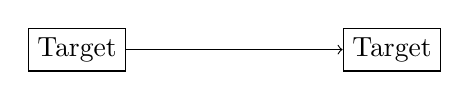
\begin{tikzpicture}
    \path ( 0, 0) node [draw] (tw) {Target};
    \path ( 4, 0) node [draw] (te) {Target};
    \draw [->] (tw.east) -- (te.west);
\end{tikzpicture}
\end{frame}

\section{Hardware Perform Future}
\begin{frame}{Hardware Perform Future}
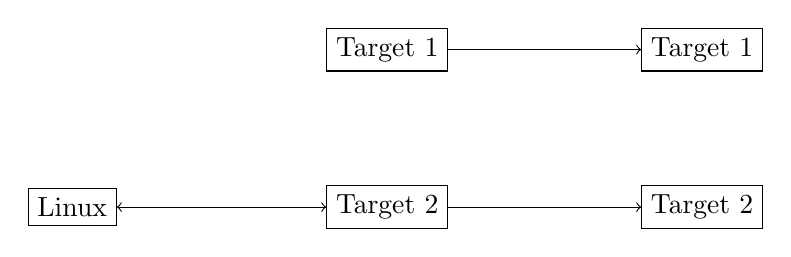
\begin{tikzpicture}
    \path ( 0, 0) node [draw] (tw1) {Target 1};
    \path ( 4, 0) node [draw] (te1) {Target 1};
    \draw [->] (tw1.east) -- (te1.west);
    \path ( 0,-2) node [draw] (tw2) {Target 2};
    \path ( 4,-2) node [draw] (te2) {Target 2};
    \draw [->] (tw2.east) -- (te2.west);
    \path (-4,-2) node [draw] (l) {Linux};
    \draw [<->] (l.east) -- (tw2.west);
\end{tikzpicture}
\end{frame}


\end{document}
